\documentclass[11pt,a4paper]{article}
\usepackage[utf8]{inputenc}
\usepackage[margin=1in]{geometry}
\usepackage{graphicx}
\usepackage{hyperref}
\usepackage{listings}
\usepackage{xcolor}
\usepackage{amsmath}
\usepackage{tikz}
\usetikzlibrary{positioning,shapes}
\usepackage{float}
\usepackage{enumitem}
\usepackage{fancyhdr}

% Code listing settings
\lstset{
    backgroundcolor=\color{gray!10},
    basicstyle=\ttfamily\small,
    keywordstyle=\color{blue},
    commentstyle=\color{green!60!black},
    stringstyle=\color{red},
    numbers=left,
    numberstyle=\tiny\color{gray},
    frame=single,
    breaklines=true,
    captionpos=b
}

% Header and footer
\pagestyle{fancy}
\fancyhf{}
\rhead{EE782 Assignment 2}
\lhead{AI Room Guard Agent}
\cfoot{\thepage}
\setlength{\headheight}{14pt}

\title{\textbf{AI Room Guard Agent: An Integrated Multi-Modal Security System}}
\author{Navaneet\footnote{This assignment was done individually by me and not as a team of two as I could not find a partner with matching timings along with complementary skills.}}
\date{\today}

\begin{document}

\maketitle

% % \tableofcontents
% \newpage

\section{Introduction}
This report details the design, implementation, and evaluation of the AI Room Guard Agent as part of the EE782 - Assignment 2. The key features of the system include
\begin{itemize}
    \item \textbf{Voice Activation}: "Guard my room" command activation
    \item \textbf{Face Recognition}: Trusted user enrollment and verification
    \item \textbf{Trust Management}: Dynamic trust scoring system
    \item \textbf{Escalating Dialogue}: Three-level conversation system
    \item \textbf{Smart Logging}: Event-based logging with spam reduction
    \item \textbf{Concurrent Processing}: Non-blocking audio and video processing
\end{itemize}

\section{System Architecture}


The overall architecture of the AI Room Guard Agent is modular as illustrated in Figure \ref{fig:architecture}. The functionality of the core components is described in further subsections.
\begin{figure}[H]
\centering
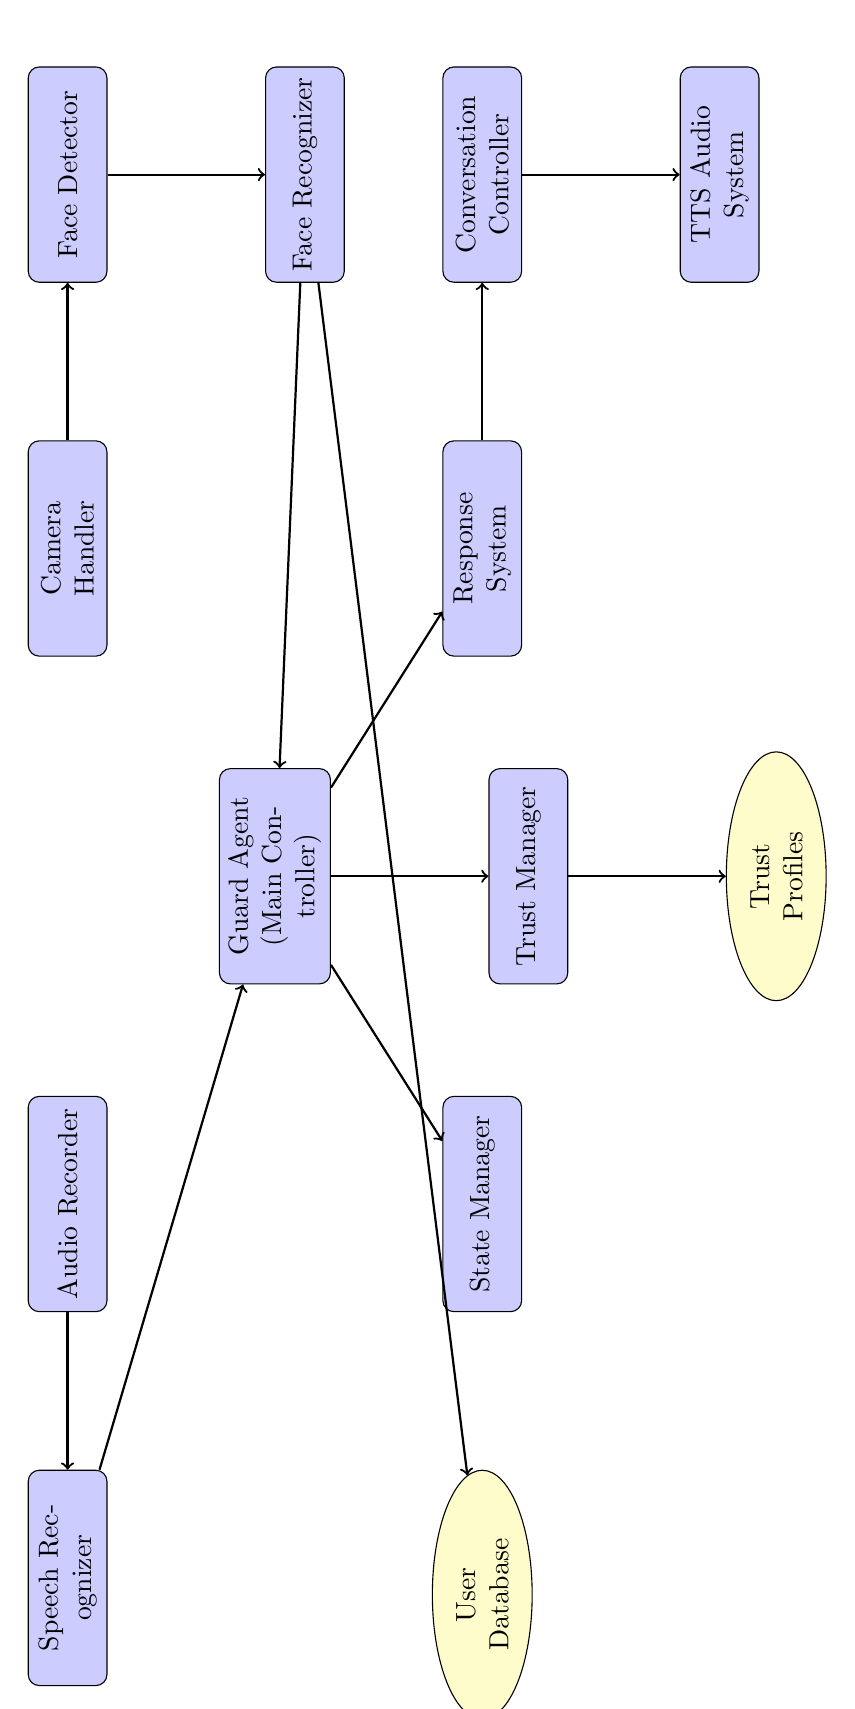
\begin{tikzpicture}[node distance=2cm, auto,rotate=90,transform shape]

    % Define styles
    \tikzstyle{component} = [rectangle, draw, fill=blue!20, text width=2.5cm, text centered, rounded corners, minimum height=1cm]
    \tikzstyle{data} = [ellipse, draw, fill=yellow!20, text width=2cm, text centered, minimum height=0.8cm]
    \tikzstyle{flow} = [thick, ->]
    
    % Core components
    \node [component] (guard) {Guard Agent\\(Main Controller)};
    
    % Audio components
    \node [component, above left=of guard] (audio_rec) {Audio Recorder};
    \node [component, left=of audio_rec] (speech_rec) {Speech Recognizer};
    
    % Video components
    \node [component, above right=of guard] (camera) {Camera Handler};
    \node [component, right=of camera] (face_det) {Face Detector};
    \node [component, below=of face_det] (face_rec) {Face Recognizer};
    
    % Core logic
    \node [component, below left=of guard] (state) {State Manager};
    \node [component, below=of guard] (trust) {Trust Manager};
    \node [component, below right=of guard] (response) {Response System};
    
    % Conversation system
    \node [component, right=of response] (conv) {Conversation\\Controller};
    \node [component, below=of conv] (tts) {TTS Audio\\System};
    
    % Data stores
    \node [data, left=of state] (user_db) {User\\Database};
    \node [data, below=of trust] (trust_db) {Trust\\Profiles};
    
    % Flows
    \draw [flow] (audio_rec) -> (speech_rec);
    \draw [flow] (speech_rec) -> (guard);
    \draw [flow] (camera) -> (face_det);
    \draw [flow] (face_det) -> (face_rec);
    \draw [flow] (face_rec) -> (guard);
    \draw [flow] (guard) -> (state);
    \draw [flow] (guard) -> (trust);
    \draw [flow] (guard) -> (response);
    \draw [flow] (response) -> (conv);
    \draw [flow] (conv) -> (tts);
    \draw [flow] (face_rec) -> (user_db);
    \draw [flow] (trust) -> (trust_db);
    
\end{tikzpicture}
\caption{AI Room Guard Agent System Architecture}
\label{fig:architecture}
\end{figure}


\subsection{Core Controller (Guard Agent)}
The central orchestrator that manages all system components and coordinates their interactions. Implements concurrent processing for audio and video streams while maintaining system state consistency.

\subsection{Audio Processing Pipeline}
\begin{itemize}
    \item \textbf{Audio Recorder}: Captures real-time audio from microphone using PyAudio
    \item \textbf{Speech Recognizer}: Converts speech to text using Google Speech Recognition API
    \item \textbf{Command Detection}: Fuzzy matching for activation commands with confidence scoring
\end{itemize}

\subsection{Vision Processing Pipeline}
\begin{itemize}
    \item \textbf{Camera Handler}: Manages webcam access and frame capture
    \item \textbf{Face Detector}: Identifies face locations using HOG-based detection
    \item \textbf{Face Recognizer}: Matches detected faces against enrolled users using face\_recognition library
\end{itemize}

\subsection{Trust and Security Management}
\begin{itemize}
    \item \textbf{Trust Manager}: Maintains dynamic trust scores for users
    \item \textbf{User Database}: Stores face encodings and user profiles
    \item \textbf{Response System}: Generates appropriate responses based on recognition results
\end{itemize}

\section{Integration Challenges and Solutions}

\subsection{Concurrency Management}

\textbf{Challenge}: Ensuring non-blocking audio and video processing while maintaining system responsiveness.

\textbf{Solution}: Implemented concurrent processing using threading with proper synchronization:

\begin{itemize}
    \item Audio processing runs in a separate thread with queue-based communication
    \item Face recognition uses timestamp-based idle periods for trusted users
    \item State management uses thread-safe locks for consistency
\end{itemize}

\subsection{Real-time Performance}

\textbf{Challenge}: Balancing recognition accuracy with real-time performance constraints.

\textbf{Solution}: Optimized processing pipeline:

\begin{itemize}
    \item Frame skipping for face detection (process every 2nd frame)
    \item Configurable face recognition intervals during escalation (5 seconds)
    \item Efficient face encoding caching and comparison
\end{itemize}

\subsection{Audio System Integration}

\textbf{Challenge}: Managing audio input/output conflicts and system compatibility.

\textbf{Solution}: Robust audio handling:

\begin{itemize}
    \item Proper PyAudio stream management with exception handling
    \item Device-specific configuration (44.1kHz sample rate)
    \item Graceful fallback to alternative TTS systems
\end{itemize}


\textbf{Challenge}: Non natural sounding voice from TTS system.

\textbf{Solution}: Use \texttt{gemini-2.0-flash-tts-preview} (partial success)

\begin{itemize}
    \item \texttt{gemini-2.0-flash-tts-preview} produces more natural sounding voice
    \item It also supports changing the tone of the voice for an angry or stern response
    \item The problem is however that the API rate limits are stingy
\end{itemize}

\subsection{Internet Dependency}

\textbf{Challenge}: IITB internet has become ever more unreliable.

\textbf{Solution}: 
\begin{itemize}
    \item Fallback to offline TTS (whisper) on speech recognition API call failure
    \item Fallback to hard coded excalation messages on LLM API call failure 
\end{itemize}

\section{Testing Results}

\subsection{Voice Activation Accuracy}

The speech recognition system accuracy is rougly:

\begin{table}[H]
\centering
\begin{tabular}{|l|c|c|c|}
\hline
\textbf{Command} & \textbf{Tests} & \textbf{Successful} & \textbf{Accuracy} \\
\hline
``Guard my room'' & 20 & 12 & 60\% \\
``Activate surveillance'' & 20 & 19 & 95\% \\
``Start surveillance'' & 20 & 18 & 90\% \\
\end{tabular}
\caption{Voice Activation Test Results}
\end{table}

\subsection{Face Recognition Performance}

Face recognition testing was conducted under various conditions:

\begin{table}[H]
\centering
\begin{tabular}{|l|c|c|c|}
\hline
\textbf{Condition} & \textbf{Tests} & \textbf{Correct ID} & \textbf{Accuracy} \\
\hline
Good lighting & 15 & 14 & 93\% \\
Low lighting & 15 & 10 & 67\% \\
Different angles & 15 & 13 & 87\% \\
\end{tabular}
\caption{Face Recognition Test Results}
\end{table}

\subsection{System Integration Testing}

End-to-end system testing demonstrated successful integration:

\begin{itemize}
    \item \textbf{Activation Flow}: Voice command → Camera activation → Face detection (Success: ~95\%)
    \item \textbf{Trust User Flow}: Face recognition → Trust update → Welcome message (Success: ~95\%)
    \item \textbf{Deactivation Flow}: "Stop" command → System shutdown (Success: ~90\%)* 
\end{itemize}
* Sometimes the "stop" command is not recognized, probably getting skipped as all other systems are hogging responses.
\section{Ethical Considerations}

\subsection{Privacy Protection}

\begin{itemize}
    \item \textbf{Consent}: I have enrolled only myself as a trusted user. For conducting escalation on a stranger, I showed a face image on my phone to the camera. The image was taken from "labelled faces in the wild" dataset.
    \item \textbf{Data Storage}: Face data is stored locally. Identification is also done locally.
    \item \textbf{Deletion}: The enrolled face data can be deleted very easily.
\end{itemize}

\subsection{Security Considerations}

\begin{itemize}
    \item \textbf{Spoofing Protection}: Photo-based attacks is not prevented, but can be mitigated with liveness detection in future.
    \item \textbf{Audit Trail}: Comprehensive logging of all security events
\end{itemize}

\section{Performance Analysis}

\subsection{Resource Utilization}

System resource usage during operation:

\begin{table}[H]
\centering
\begin{tabular}{|l|c|c|c|}
\hline
\textbf{Component} & \textbf{CPU Usage} & \textbf{Memory Usage} & \textbf{Response Time} \\
\hline
Face Detection & 15-25\% & 150MB & 200ms \\
Speech Recognition & 5-10\% & 80MB & 500ms \\
Face Recognition & 10-20\% & 100MB & 300ms \\
TTS Generation & 20-30\% & 120MB & 800ms \\
Overall System & 30-45\% & 350MB & 1.2s \\
\hline
\end{tabular}
\caption{System Resource Utilization}
\end{table}


\subsection{Lessons Learned}

\begin{itemize}
    \item Integration complexity increases exponentially with number of modalities
    \item Real-time constraints require careful optimization and concurrent design
    \item Comprehensive logging and monitoring are essential for understanding what is going on inside
\end{itemize}
\end{document}